\section{Zielsetzung}

In diesem Versuch sollen durch verschiedene Brückenschaltungen unbekannte Widerstände gemessen, 
sowie eine Klirrfaktorbestimmung durchgeführt werden.

\section{Theoretische Grundglage}

\begin{figure}
            \centering
               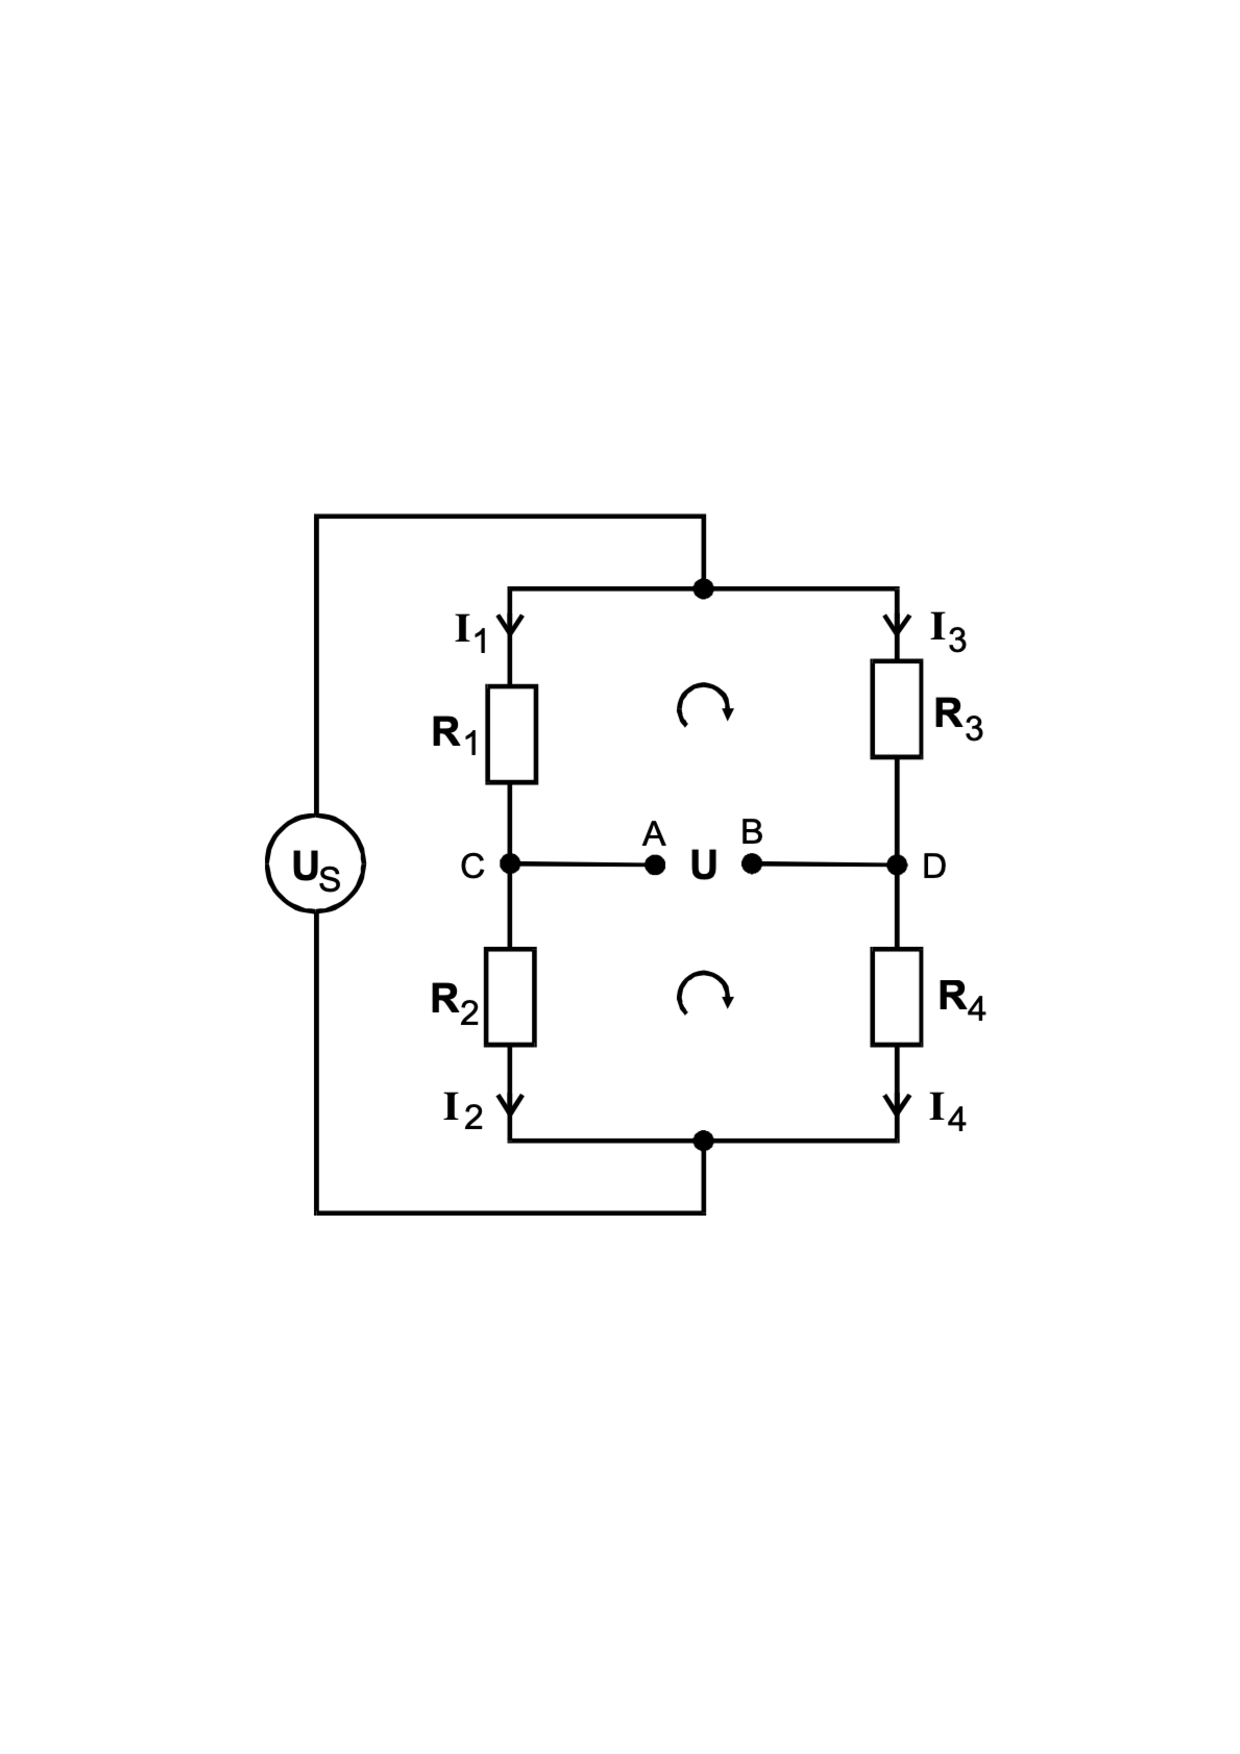
\includegraphics[height=7cm]{prinz.pdf}
               \caption{Prinzipielle Brückenschaltung.}
               \label{fig:prinz}
        \end{figure}

\noindent 
In der Abbildung (\ref{fig:prinz}) ist der Aufbau einer prinzipiellen Brückenschaltung dargestellt.
Hier wird die Potentialdifferenz zwischen den Punkten A und B, die Brückenspannung genannt wird, in Abhängigkeit ihrer Widerstandsverhältnissen untersucht.
Um die Brückenspannung zu berechnen wird sich auf die Kirchhoff'schen Gesetze berufen.
Diese Lauten wie folgt:

\noindent
\begin{enumerate}
\item \textbf{Knotenpunktsatz}

In jedem Verzweigungspunkt (Knotenpunkt) eines Stromkreises ist die Summe der zufließenden Ströme ($\text{I}>0$) gleich der Summe der abfließenden Ströme ($\text{I}<0$).

\begin{equation}
\sum_\text{k} \text{I}_\text{k} = 0
\label{eqn:knotenpunktsatz}
\end{equation}

\item \textbf{Maschensatz}

In einem unverzweigten Stromkreis bzw. in jeder Masche ist die Summe aller Spannungsabfälle $\text{U}_\text{k}$ 
gleich der Summe der Produkte aus den Stromstärken $\text{I}_\text{k}$ und den Widerständen $\text{R}_\text{k}$.

\begin{equation}
\sum_\text{k} \text{U}_\text{k} = \sum_\text{k} \text{I}_\text{k} \, \text{R}_\text{k}
\label{eqn:maschensatz}
\end{equation}
\end{enumerate}

\newpage \noindent
Mithilfe des 1. Kirchhoff'schen Gesetzes (\ref{eqn:knotenpunktsatz}) ergibt sich für Abbildung (\ref{fig:prinz}), dass über die Brücke A - B kein Strom fließt:

\begin{equation}
\text{I}_1=\text{I}_2 
\label{eqn:i1}
\end{equation}

\noindent
und

\begin{equation}
\text{I}_3=\text{I}_4 
\label{eqn:i3}
\end{equation}

\noindent
Das 2. Kirchhoff'sche Gesetz (\ref{eqn:maschensatz}) liefert für die beiden Maschen in Abbildung (\ref{fig:prinz})

\begin{equation}
\text{U} = -\text{R}_1 \text{I}_1 + \text{R}_3 \text{I}_3
\label{eqn:u1}
\end{equation}

\noindent
und

\begin{equation}
-\text{U} = -\text{R}_2 \text{I}_2 + \text{R}_4 \text{I}_4  .
\label{eqn:u2}
\end{equation}

\noindent
Wird für (\ref{eqn:u2}) genutzt, dass Gleichung (\ref{eqn:i1}) und (\ref{eqn:i3}) gilt, ergibt sich

\begin{equation}
-\text{U} = -\text{R}_2 \text{I}_1 + \text{R}_4 \text{I}_3  .
\label{eqn:u3}
\end{equation}

\noindent
Aus Gleichung (\ref{eqn:u3}) und (\ref{eqn:u1}) folgt nun

\begin{equation}
\text{U} = \frac{\text{R}_2 \text{R}_3 - \text{R}_1 \text{R}_4}{\text{R}_3 + \text{R}_4} \text{I}_1
\label{eqn:u4}
\end{equation}

\noindent
Außerdem lässt sich die Speisespannung $\text{U}_\text{S}$ nach (\ref{eqn:maschensatz}) ausdrücken

\begin{equation}
\text{U}_\text{S} = \text{I}_1 (\text{R}_1 + \text{R}_2) 
\label{eqn:us}
\end{equation}

\noindent
und kann nach $\text{I}_1$ umgestellt in (\ref{eqn:u4}) eingesetzt werden. 
Dann gilt:

\begin{equation}
\text{U} = \frac{\text{R}_2 \text{R}_3 - \text{R}_1 \text{R}_4}{(\text{R}_3 + \text{R}_4)(\text{R}_1 + \text{R}_2)} \text{U}_\text{S}
\label{eqn:ub}
\end{equation}

\noindent
Dies ist ein Ausdruck für die Brückenspannung. 
Diese verschwindet, wenn

\begin{equation}
\text{R}_2 \text{R}_3 = \text{R}_1 \text{R}_4
\label{eqn:abgleichbed}
\end{equation}

\noindent
ist, was auch als abgeglichene Brücke bezeichnet wird.
Aus der Abgleichbedingung kann nun ein unbekannter Widerstand durch Variierung der bekannten drei anderen Widerständen gemessen werden,
indem versucht wird, die Brückenspannung verschwinden zu lassen. 

\newpage
\subsection{Brückenschaltungen mit komplexen Widerständen}

\noindent
Sobald sich in einer Schaltung Kapazitäten und Induktivitäten befinden, ist es nötig, mit komplexen Widerständen zu rechnen.
Ein komplexer Widerstand lässt sich allgemein in folgender Form darstellen:

\begin{equation}
\symfrak{R} = \text{X} + \text{jY}  .
\label{eqn:rkomplex}
\end{equation}

\noindent
Dabei ist X der Wirkwiderstand, Y der Blindwiderstand und j die imaginäre Einheit.
Die Widerstände einer Induktivität L, einer Kapazität C und eines ohmschen Widerstandes R lassen sich auch in dieser Weise mit $\omega$ als Kreisfrequenz darstellen.

\begin{equation}
\symfrak{R}_\text{C} = -\frac{\text{j}}{\omega \text{C}}
\label{eqn:r_c}
\end{equation}

\begin{equation}
\symfrak{R}_\text{L} = \text{j}\omega\text{L}
\label{eqn:r_l}
\end{equation}

\begin{equation}
\symfrak{R}_\text{R} = \text{R}
\label{eqn:r_r}
\end{equation}

\noindent
Nach Gleichung (\ref{eqn:abgleichbed}) ist die Abgleichbedingung für eine Brücke mit komplexen Widerständen 

\begin{equation}
\symfrak{R}_2 \symfrak{R}_3 = \symfrak{R}_1 \symfrak{R}_4 .
\label{eqn:abgleichbedkom}
\end{equation}

\noindent
Damit die komplexe Abgleichbedingung (\ref{eqn:abgleichbedkom}) erfüllt ist, müssen Real- und Imaginärteil auf beiden Seiten gleich sein.
Daraus ergeben sich zwei Bedingungen, die bei einer abgeglichenen Wechselstrombrücke gleichzeitig erfüllt sein müssen:

\begin{equation}
\text{X}_1 \text{X}_4 - \text{Y}_1 \text{Y}_4 = \text{X}_2 \text{X}_3 - \text{Y}_2 \text{Y}_3
\label{eqn:abgleichbed1}
\end{equation}

\noindent
und 

\begin{equation}
\text{X}_1 \text{Y}_4 + \text{X}_4 \text{Y}_1 = \text{X}_2 \text{Y}_3 \text{X}_3 \text{Y}_2  .
\label{eqn:abgleichbed2}
\end{equation}

\newpage
\subsection{Beschreibung spezieller Brückenschaltungen}

\subsubsection{Wheatstonesche Brückenschaltung}

\begin{figure}
            \centering
               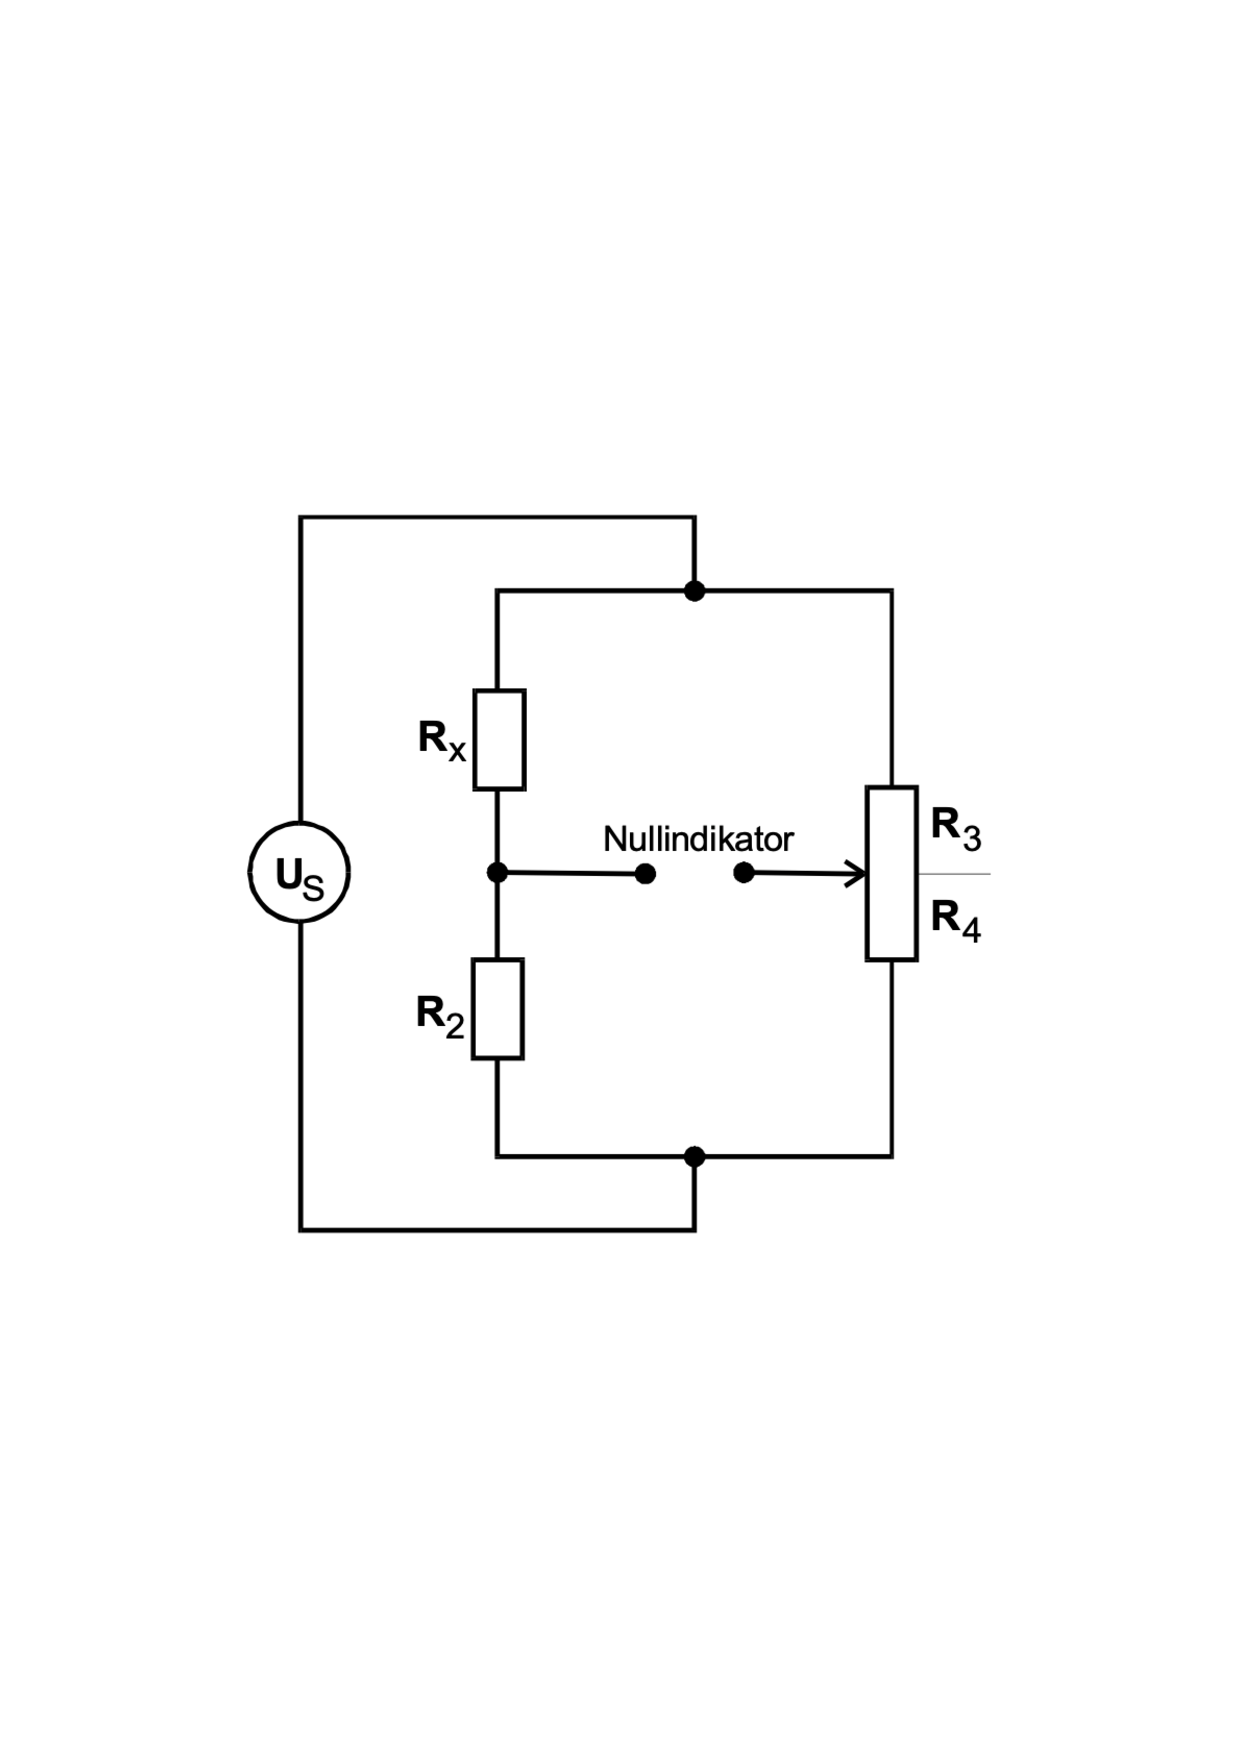
\includegraphics[height=7cm]{wheatstone.pdf}
               \caption{Wheatstonesche Brückenschaltung.}
               \label{fig:wheat}
        \end{figure}

\noindent
Da die Wheatstonesche Brückenschaltung nur ohmsche Widerstände enthält, kann sie sowohl mit Gleichstrom, 
als auch mit Wechselstrom betrieben werden.
Sie ist wie in Abbildung (\ref{fig:wheat}) dargestellt aufgebaut und kann zur Bestimmung eines unbekannten Widerstandes $\text{R}_\text{X}$ verwendet werden.
Nach der Abgleichbedingung (\ref{eqn:abgleichbed}) kann $\text{R}_\text{X}$ durch

\begin{equation}
\text{R}_\text{X} = \text{R}_2 \frac{\text{R}_3}{\text{R}_4}
\end{equation}

\noindent
bestimmt werden, wobei das Verhältnis von $\text{R}_3$ zu $\text{R}_4$ durch ein Potentiometer realisiert wird.

\subsubsection{Kapazitätsmessbrücke}
Da bei einem realen Kondensator dielektrische Verluste auftreten, wird im Ersatzschaltbild ein ohmscher Widerstand in Reihe geschaltet, sodass gilt:

\begin{equation}
\symfrak{R}_\text{Creal}= \text{R}-\frac{\text{j}}{\omega \text{C}}
\label{eqn:r_creal}
\end{equation}

\noindent
Eine Kapazitätsmessbrücke, mit eine unbekannte Kapazität $\text{C}_\text{X}$ gemessen werden kann, ist in Abbilung (\ref{fig:kap}) dargestellt.

\newpage
\begin{figure}
            \centering
               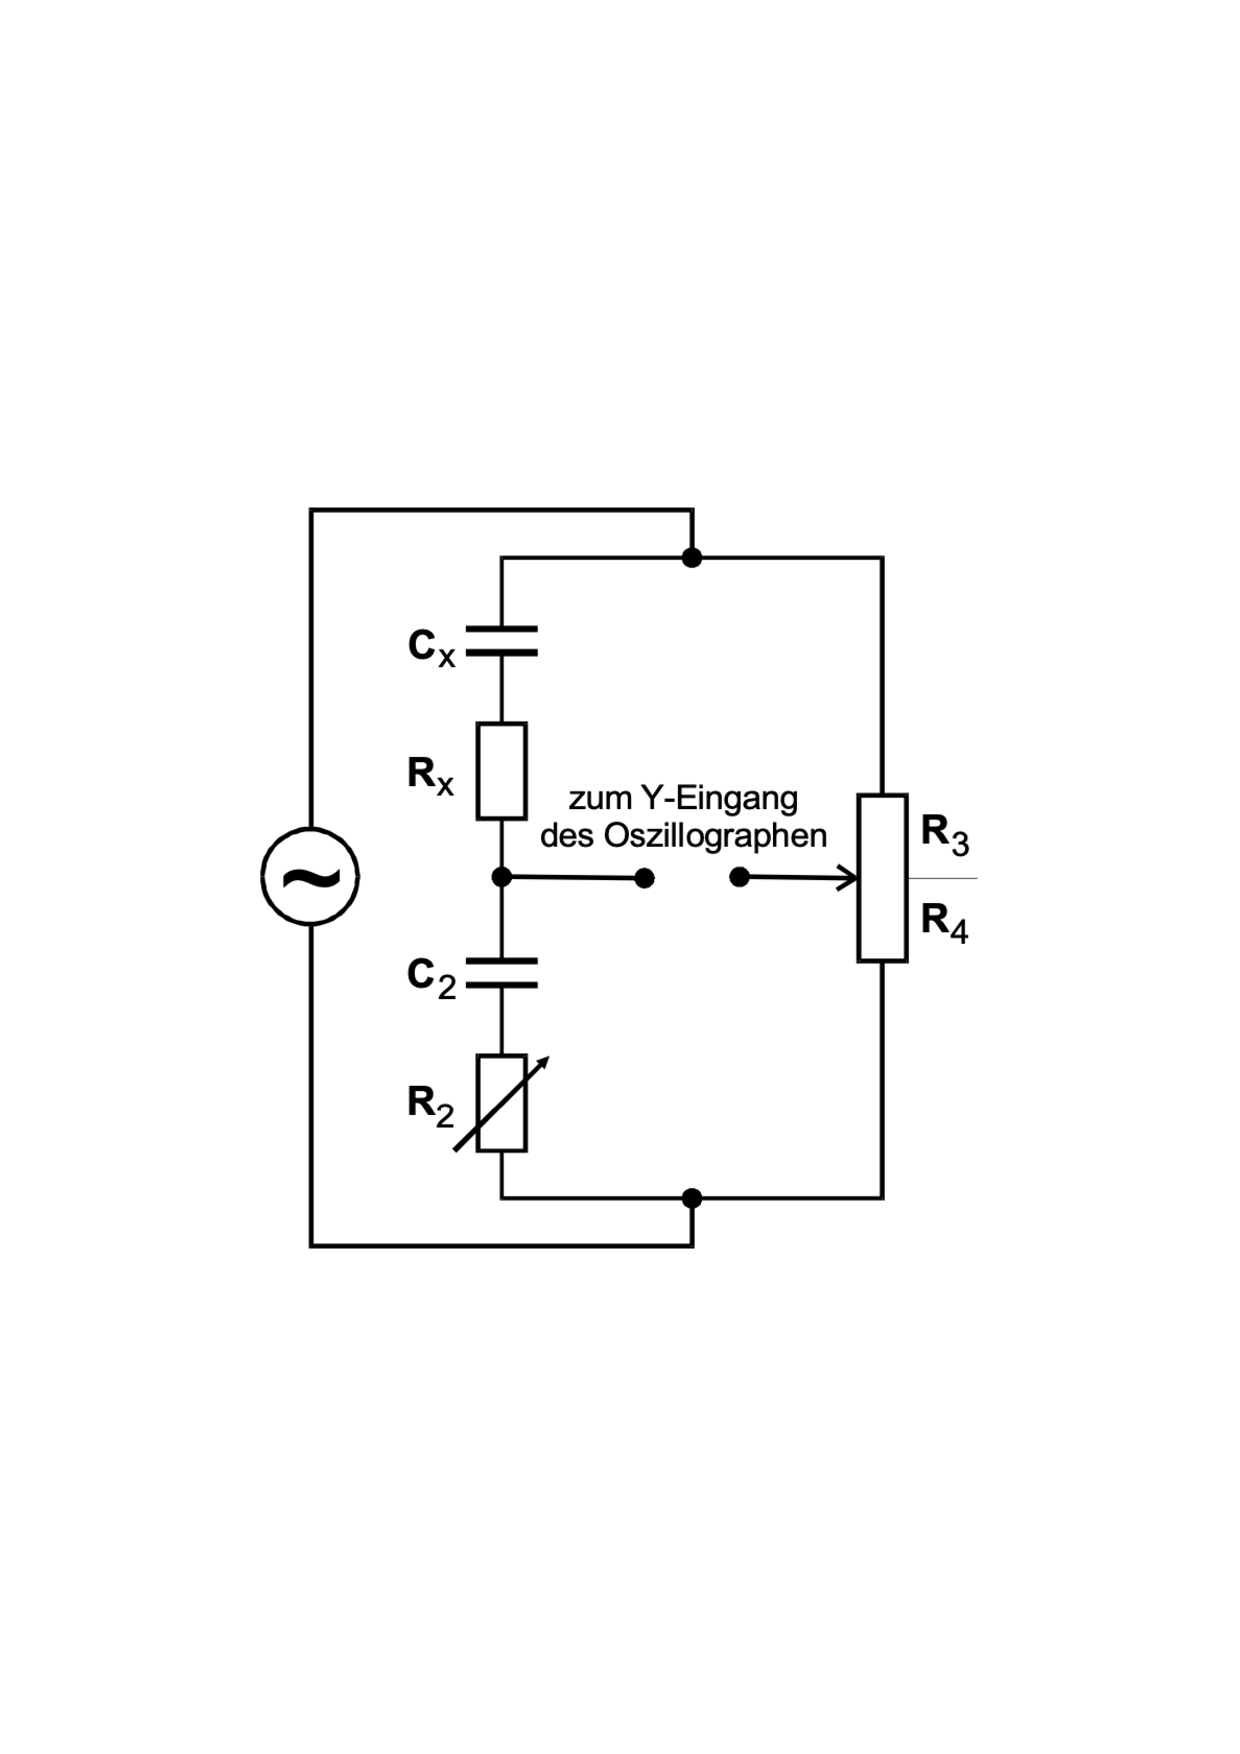
\includegraphics[height=7cm]{kapazitaet.pdf}
               \caption{Kapazitätsmessbrücke für realen Kondensator.}
               \label{fig:kap}
        \end{figure}

\noindent
Um $\text{C}_\text{X}$ und $\text{R}_\text{X}$ zu bestimmen müssen die Abgleichbedingungen (\ref{eqn:abgleichbed1}) und (\ref{eqn:abgleichbed2}) mit

\begin{align*}
\text{Y}_1 &= -\frac{1}{\omega\text{C}_\text{X}}\\
\text{Y}_2 &= -\frac{1}{\omega\text{C}_2}\\
\text{Y}_3 &= \text{Y}_4 = 0
\end{align*}

\noindent
berücksichtigt werden.
Daraus ergeben sich die Gleichungen

\begin{equation}
\text{R}_\text{X} = \text{R}_2 \frac{\text{R}_3}{\text{R}_4}
\label{eqn:r_x}
\end{equation}

\noindent
und 

\begin{equation}
\text{C}_\text{X} = \text{C}_2 \frac{\text{C}_3}{\text{C}_4}  .
\label{eqn:c_x}
\end{equation}

\subsubsection{Induktivitätsmessbrücke}
Die Induktivitätsmessbrücke ist analog zur Kapazitätsmessbrücke aufgebaut.
Auch hier wird zu jeder Induktivität ein ohmscher Widerstand aufgrund von Wärmeverlusten in Reihe geschaltet, mit

\begin{equation}
\symfrak{R}_\text{Lreal}= \text{R}+\text{j} \omega \text{L}  
\label{eqn:r_lreal}
\end{equation}

\begin{align*}
\text{Y}_1 &= \omega\text{L}_\text{X}\\
\text{Y}_2 &= \omega\text{L}_2\\
\shortintertext{und}
\text{Y}_3 &= \text{Y}_4 = 0  .
\end{align*}

\noindent
Der Aufbau hat die in Abbildung (\ref{fig:induktiv})
gezeigte Gestalt.

\begin{figure}
            \centering
               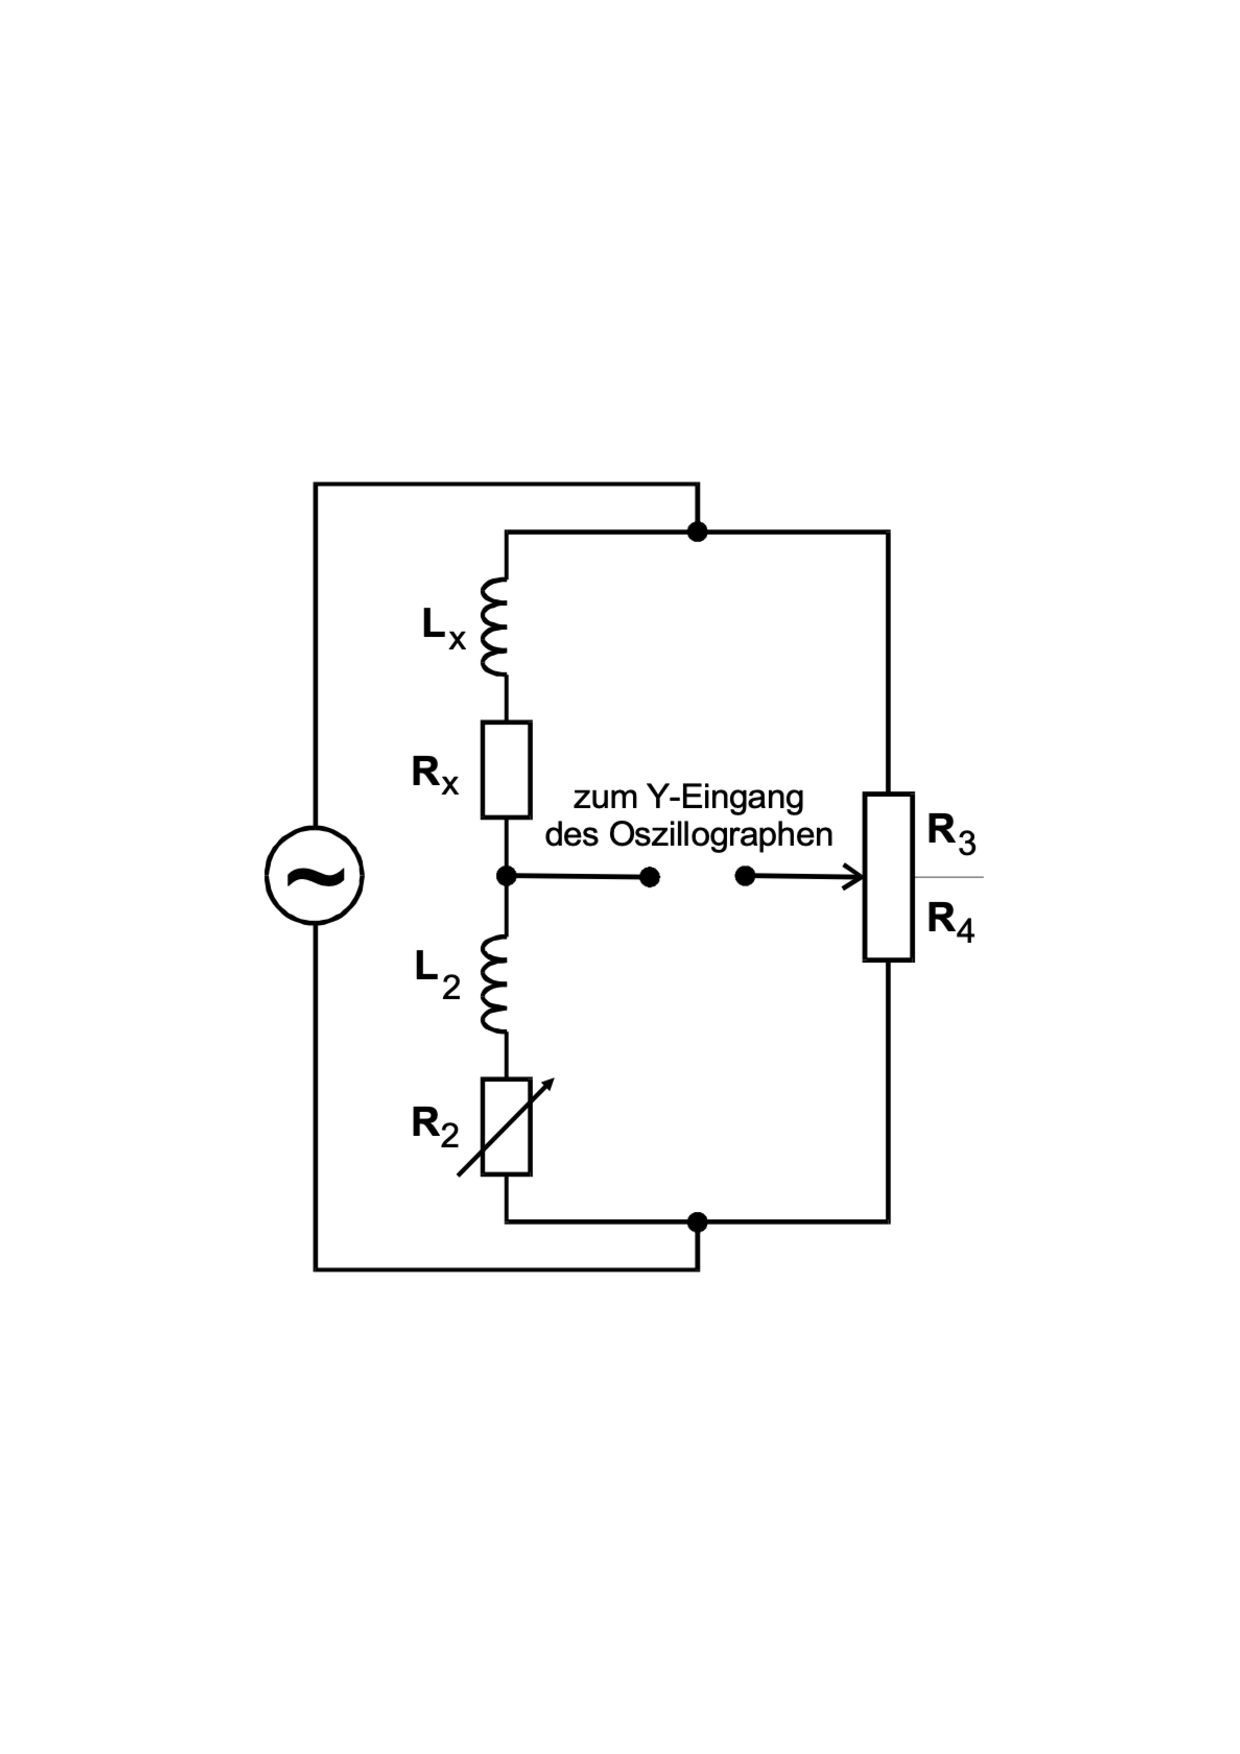
\includegraphics[height=7cm]{induktiv.pdf}
               \caption{Induktivitätsmessbrücke für reale Spule.}
               \label{fig:induktiv}
        \end{figure}

\noindent
Die Abgleichbedingung lauten nach (\ref{eqn:abgleichbed1}) und (\ref{eqn:abgleichbed2})

\begin{equation}
\text{R}_\text{X} = \text{R}_2 \frac{\text{R}_3}{\text{R}_4}
\label{eqn:r_x}
\end{equation}

\noindent
und 

\begin{equation}
\text{L}_\text{X} = \text{L}_2 \frac{\text{L}_3}{\text{L}_4}  .
\label{eqn:c_x}
\end{equation}

\noindent
Dabei sollte der Wirkanteil in dem Brückenzweig mit $\text{L}_2$ allein durch den Regelwiderstand $\text{R}_2$ realisiert werden.
Da dies insbesondere für kleine Frequenzen schwer umzusetzen ist, wird weiter noch die Maxwell-Brücke betrachtet, 
bei der anstelle von $\text{L}_2$ eine Normalkapazität verwendet wird.

\subsubsection{Induktivitätsmessung durch Maxwell-Brücke}

\noindent
Bei einer Maxwell-Brücke sind die Abgleichelemente die Regelwiderstände $\text{R}_3$ und $\text{R}_4$.
$\text{R}_2$ ist ein bekannter Widerstand mit einer möglichst engen Toleranz und $\text{C}_4$ eine möglichst verlustarme Kapazität.

\begin{figure}
            \centering
               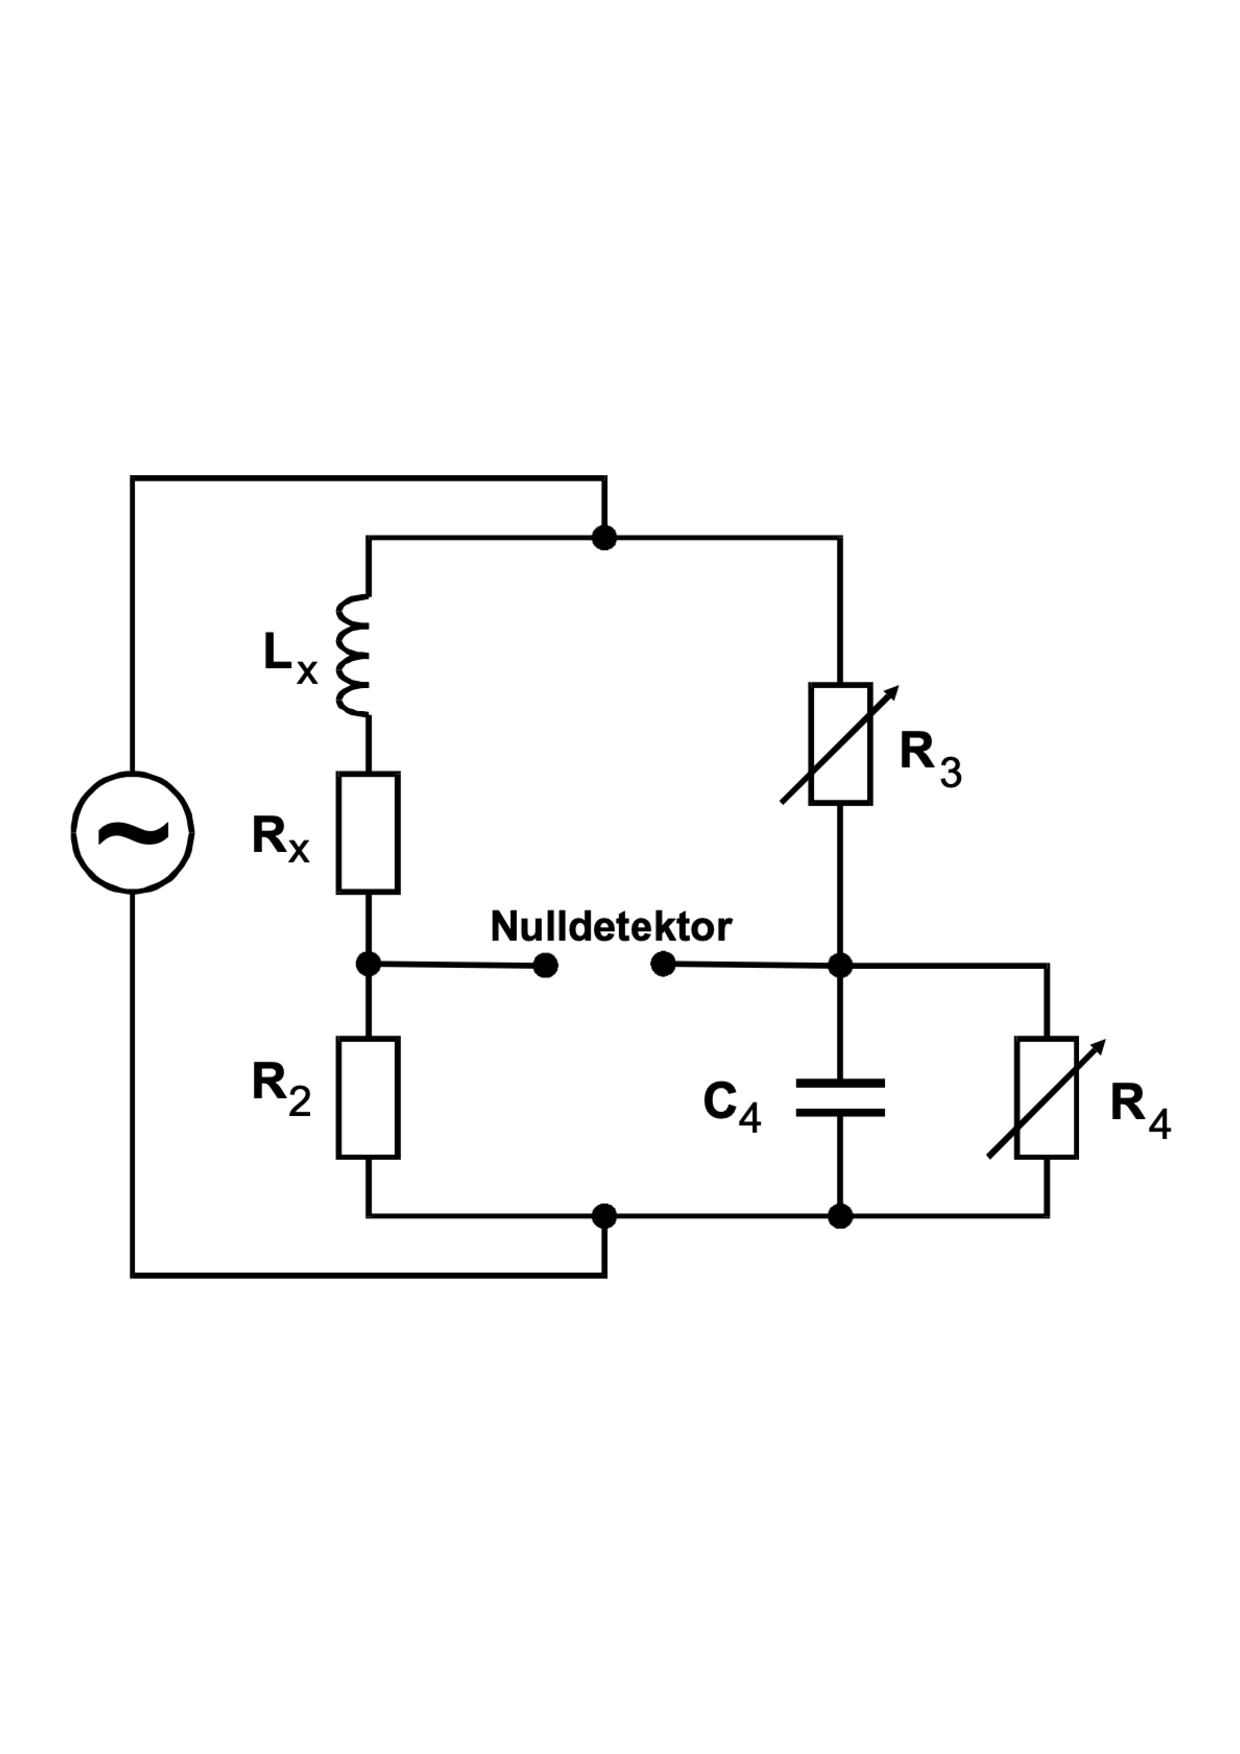
\includegraphics[height=7cm]{maxwell.pdf}
               \caption{Maxwell-Brücke für realen Kondensator mit RC Netzwerk.}
               \label{fig:max}
        \end{figure}
 
\noindent
Mithilfe von Abbildung (\ref{fig:max}) lassen sich die Widerstandsoperatoren bestimmen:

\begin{equation}
\symfrak{R}_1= \text{R}_\text{X}+\text{j} \omega \text{L}_\text{X}
\end{equation}

\noindent
und

\begin{equation}
\frac{1}{\symfrak{R}_4}= \frac{1}{\text{R}_4}+\text{j} \omega \text{C}_4
\end{equation}

\noindent
bzw.

\begin{equation}
\symfrak{R}_4 = \frac{\text{R}_4 - \text{j} \omega \text{C}_4 \text{R}_4^2}{1 + \omega^2 \text{C}_4^2 \text{R}_4^2}
\end{equation}

\noindent
Damit lassen sich wieder die Abgleichbedingungen nach (\ref{eqn:abgleichbed1}) und (\ref{eqn:abgleichbed2}) bestimmen.

\begin{equation}
\text{R}_\text{X} \text{R}_4 + \omega^2 \text{C}_4 \text{R}_4^2 \text{L}_\text{X} = \text{R}_2 \text{R}_3 (1 + \omega^2 \text{C}_4^2 \text{R}_4^2)
\label{eqn:abmax1}
\end{equation}

\begin{equation}
- \omega \text{R}_\text{X} \text{R}_4^2 \text{C}_4 + \omega \text{R}_4 \text{L}_\text{X} = 0
\label{eqn:abmax2}
\end{equation}

\noindent
Wird (\ref{eqn:abmax2}) nach $\text{L}_\text{X}$ umgestellt und in (\ref{eqn:abmax1}) eingesetzt, ergibt sich nach einfachen Umformungen

\begin{equation}
\text{R}_\text{X} = \text{R}_2 \frac{\text{R}_3}{\text{R}_4}
\end{equation}

\noindent
und mit (\ref{eqn:abmax2}) 

\begin{equation}
\text{L}_\text{X} = \text{R}_2 \text{R}_3 \text{C}_4   .
\end{equation}

\noindent
Es fällt auf, dass keine bisher aufgeführte Brücke in den Abgleichbedingungen von $\omega$ abhängt.
In der Praxis gibt es aber tatsächlich einen bestimmten Frequenzbereich, in dem der Abgleich mit optimalen Vorraussetzungen durchführbar ist.
So gibt es Brückenschaltungen, die den Abgleich nur bei einer Frequenz zulassen, wie zum Beispiel die Wien-Robinson-Brücke.

\newpage
\subsubsection{Wien-Robinson-Brücke}

\noindent
Die Besonderheit der Wien-Robinson-Brücke im vergleich zu den davor aufgeführten Brücken ist, dass sie keine Abgleichelemente enthält.
Die Schaltung einer solchen Brücke ist in Abbildung (\ref{fig:wien}) dargestellt.

\begin{figure}
            \centering
               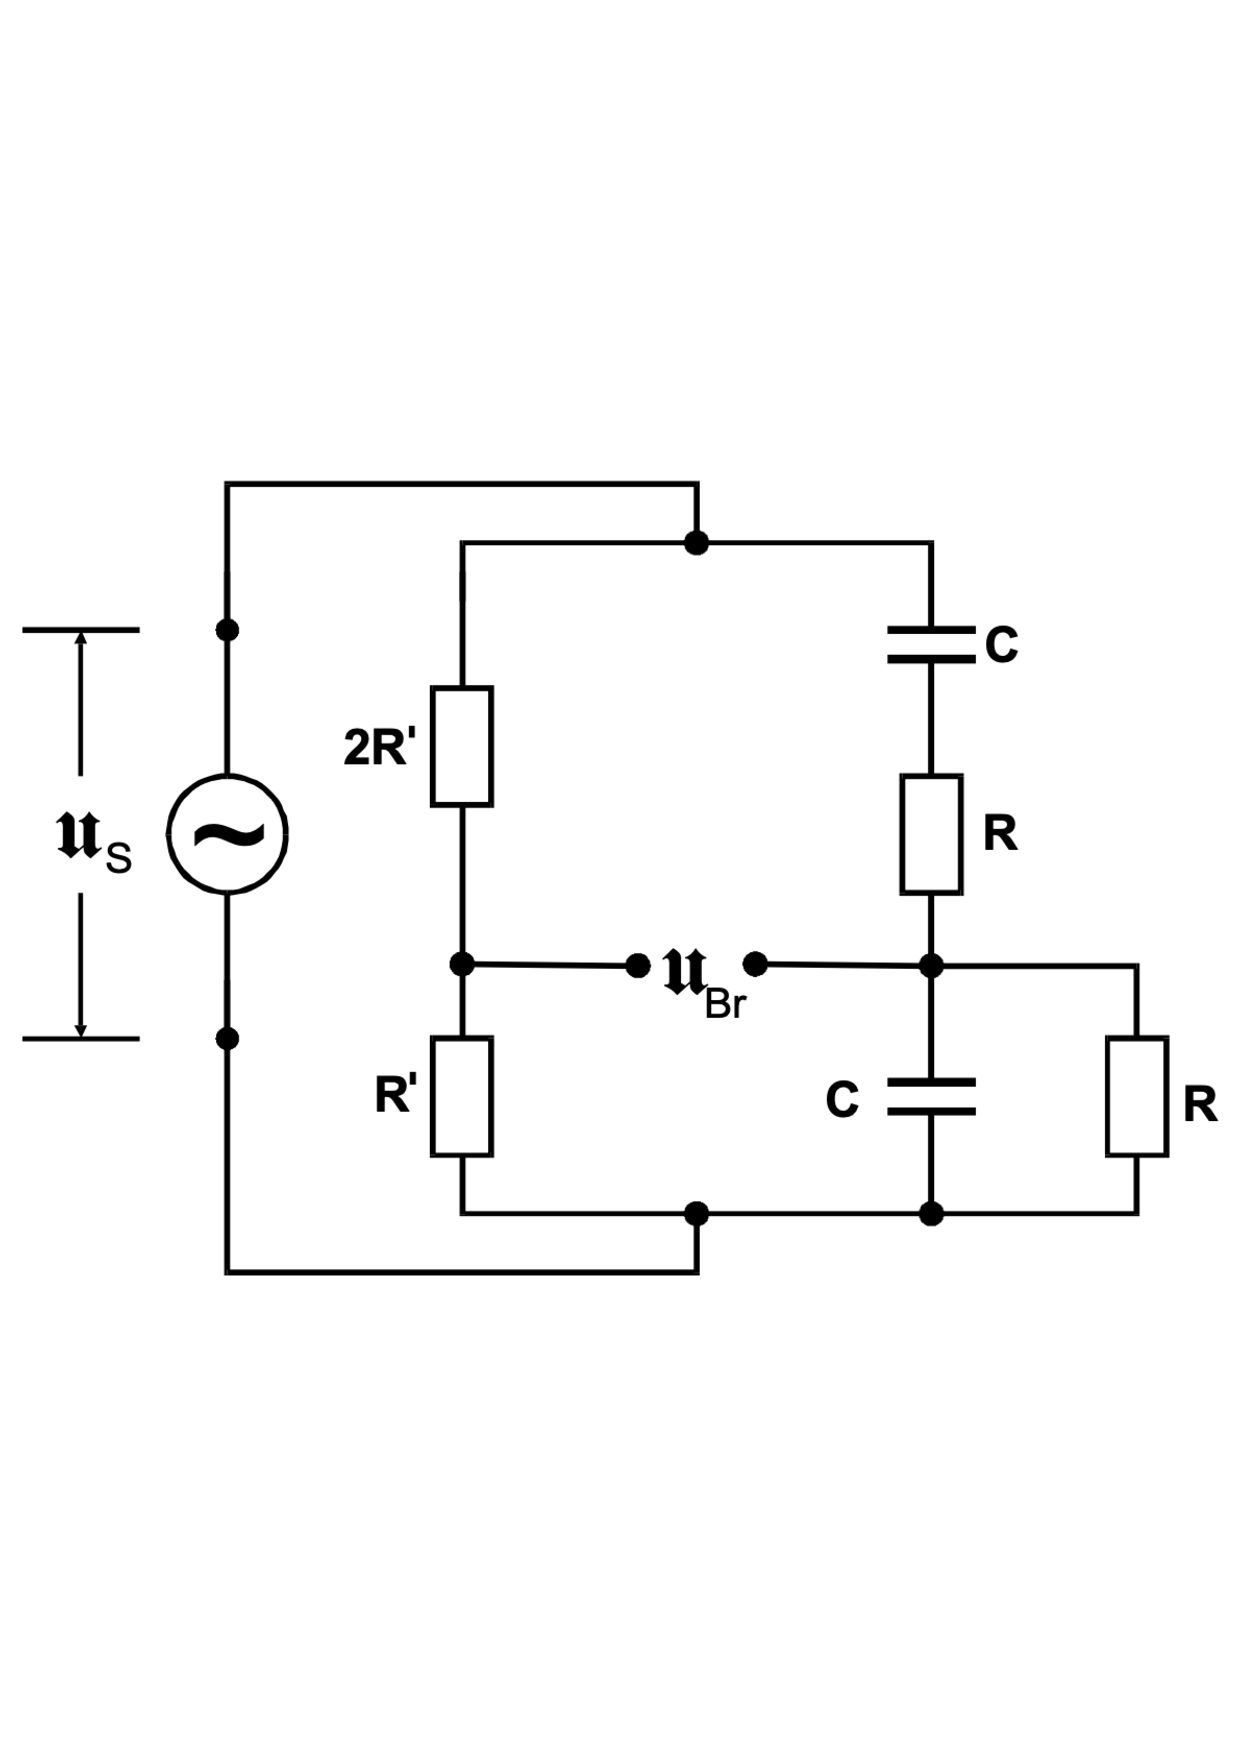
\includegraphics[height=7cm]{wien.pdf}
               \caption{Schaltung einer Wien-Robinson-Brücke.}
               \label{fig:wien}
        \end{figure}

\noindent
Das Ziel ist es zunächst, einen Ausdruck für die Brückenspannung $\symfrak{U}_\text{Br}$ in Abhängigkeit von der Frequenz zu finden.
Dazu werden die Widerstandsoperatoren aufgeführt.

\begin{align*}
\symfrak{R}_1 &= 2\text{R}' \\
\symfrak{R}_2 &= \text{R}' \\
\symfrak{R}_3 &= \text{R} + \frac{1}{\text{j} \omega \text{C}} = \frac{\text{j} \omega \text{C} \text{R} + 1}{\text{j} \omega \text{C}} \\
\symfrak{R}_4 &= \frac{\text{R}}{\text{j} \omega \text{C} \text{R} + 1}
\end{align*}

\noindent
Diese Ausdrücke können in (\ref{eqn:ub}) eingesetzt werden und weiter ergibt sich

\begin{equation}
\symfrak{U}_\text{Br} = \frac{\symfrak{R}_2 \symfrak{R}_3 - \symfrak{R}_1 \symfrak{R}_4}{(\symfrak{R}_3 + \symfrak{R}_4)(\symfrak{R}_1 + \symfrak{R}_2)} \symfrak{U}_\text{S}  .
\end{equation}

\noindent
Durch einsetzten und weiteren Umformungen folgt dann

\begin{equation}
\symfrak{U}_\text{Br} = \frac{\omega^2 \text{R}^2 \text{C}^2 - 1}{3 (1 - \omega^2 \text{R}^2 \text{C}^2) + 9 \text{j} \omega \text{R} \text{C}} \symfrak{U}_\text{S}
\end{equation}

\noindent
bzw.

\begin{equation}
\frac{\symfrak{U}_\text{S}}{\symfrak{U}_\text{Br}} = \frac{3 (1 - \omega^2 \text{R}^2 \text{C}^2) + 9 \text{j} \omega \text{R} \text{C}}{\omega^2 \text{R}^2 \text{C}^2 - 1}.
\end{equation}

\noindent 
Weitere umformungen liefern

\begin{equation}
\Bigl| \frac{\symfrak{U}_\text{Br}}{\symfrak{U}_\text{S}} \Bigr|^2 = \frac{(\omega^2 \text{R}^2 \text{C}^2 - 1)^2}{9 \{(1 - \omega^2 \text{R}^2 \text{C}^2)^2 + 9  \omega^2 \text{R}^2 \text{C}^2\}}
\label{eqn:betragub}
\end{equation}

\noindent
woraus abzulesen ist, dass die Brückenspannung genau dann verschwindet, wenn gilt:

\begin{equation}
\omega_0 = \frac{1}{\text{R} \text{C}} .
\end{equation}

\noindent 
Nun wird das Frequenzverhältnis

\begin{equation}
\Omega = \frac{\omega}{\omega_0} 
\end{equation}

\noindent
in (\ref{eqn:betragub}) eingesetzt.
Daraus ergibt sich

\begin{equation}
\Bigl| \frac{\symfrak{U}_\text{Br}}{\symfrak{U}_\text{S}} \Bigr|^2 = \frac{1}{9} \frac{(\Omega^2 - 1)^2}{(1 - \Omega^2)^2 + 9 \Omega^2} .
\label{eqn:betragub2}
\end{equation}

\noindent
Aus der Gleichung (\ref{eqn:betragub2}) kann nun abgelesen werden, dass für $\omega=\omega_0$ die Brückenspannung verschwindet
und schwächt Schwingungen in der Nähe ab.
Daran ist zu erkennen, dass die Wien-Robinson-Brücke Eigenschaften eines Filters hat.

\noindent
Mithilfe der Wien-Robinson-Brücke kann zudem eine Klirrfaktor-Messung durchgeführt werden, mit der eine Aussage über die Qualität eines Sinusgenerators getroffen werden kann.
Dabei gibt der Klirrfaktor (der im idealfall möglichst klein sein sollte) den Oberwellengehalt im Vergleich zur Grundwelle an.

\noindent
Es gilt

\begin{equation}
k = \frac{\sqrt{\text{U}_2^2 + \text{U}_3^2 + ...}}{\text{U}_1}  .
\end{equation}

\noindent
Hier ist $\text{U}_1$ die Amplitude der Grundwelle mit der Frequenz $\omega_0$ und $\text{U}_\text{n}$ die Amplitude der n-ten Oberwelle mit der Frequenz $\text{n} \omega_0$.
Zur Vereinfachung kann angenommen werden, dass die Summe der Oberwellen nur aus der zweiten Oberwelle besteht, für die 

\begin{equation}
\text{U}_2 = \frac{\text{U}_\text{Br}}{\text{f}(\Omega)}
\label{eqn:2oberwelle}
\end{equation}

\noindent
gilt.